%
%   Copyright 2013 Katarzyna Szawan <kat.szwn@gmail.com>
%       and Michał Rus <m@michalrus.com>
%
%   Licensed under the Apache License, Version 2.0 (the "License");
%   you may not use this file except in compliance with the License.
%   You may obtain a copy of the License at
%
%       http://www.apache.org/licenses/LICENSE-2.0
%
%   Unless required by applicable law or agreed to in writing, software
%   distributed under the License is distributed on an "AS IS" BASIS,
%   WITHOUT WARRANTIES OR CONDITIONS OF ANY KIND, either express or implied.
%   See the License for the specific language governing permissions and
%   limitations under the License.
%

\subsection{Data representation}
\label{subsec:data-repr}

Mind maps edited in our software will be kept in a SQL database (\cref{fig:erd}) which consists of two tables.

\begin{enumerate}
	\item The first represents a mind map with a UUID.
	\item The second --- a single `mind node' which has the following fields: \begin{itemize}
		\item UUID,
		\item its mind map's UUID,
		\item some textual content,
		\item parent node UUID,
		\item timestamp of the last modification (provided only by server, this is \emph{not a local time}; if Android modifies a node this is set to \inlinecode{NULL}; thus, local client time is \emph{never} used for synchronization protocol, as it could be set wrong),
		\item and a flag which says whether there was a merge conflict in the past, which has not yet been taken care of by the user.
	\end{itemize}
\end{enumerate}

Both local database in Android devices (SQLite) and server-side database (PostgreSQL) share the same scheme.

\todo[inline]{\igor{"co z \emph{relacjami} między node'ami niespokrewnionymi? Chodzi o kręskę między dowolnymi node'ami."}}

\todo[inline]{\igor{"co z notatkami, ikonami, załącznikami, XMind compatibility"}}

\todo[inline]{\michal{Wpisać \emph{TUTAJ jeszcze}, że nie robimy tych wszystkich bajerów, bo jak zobaczy ERD, \cref{fig:erd}, to znów to sobie przypomni!}}

\begin{figure}[h]
	\centering
	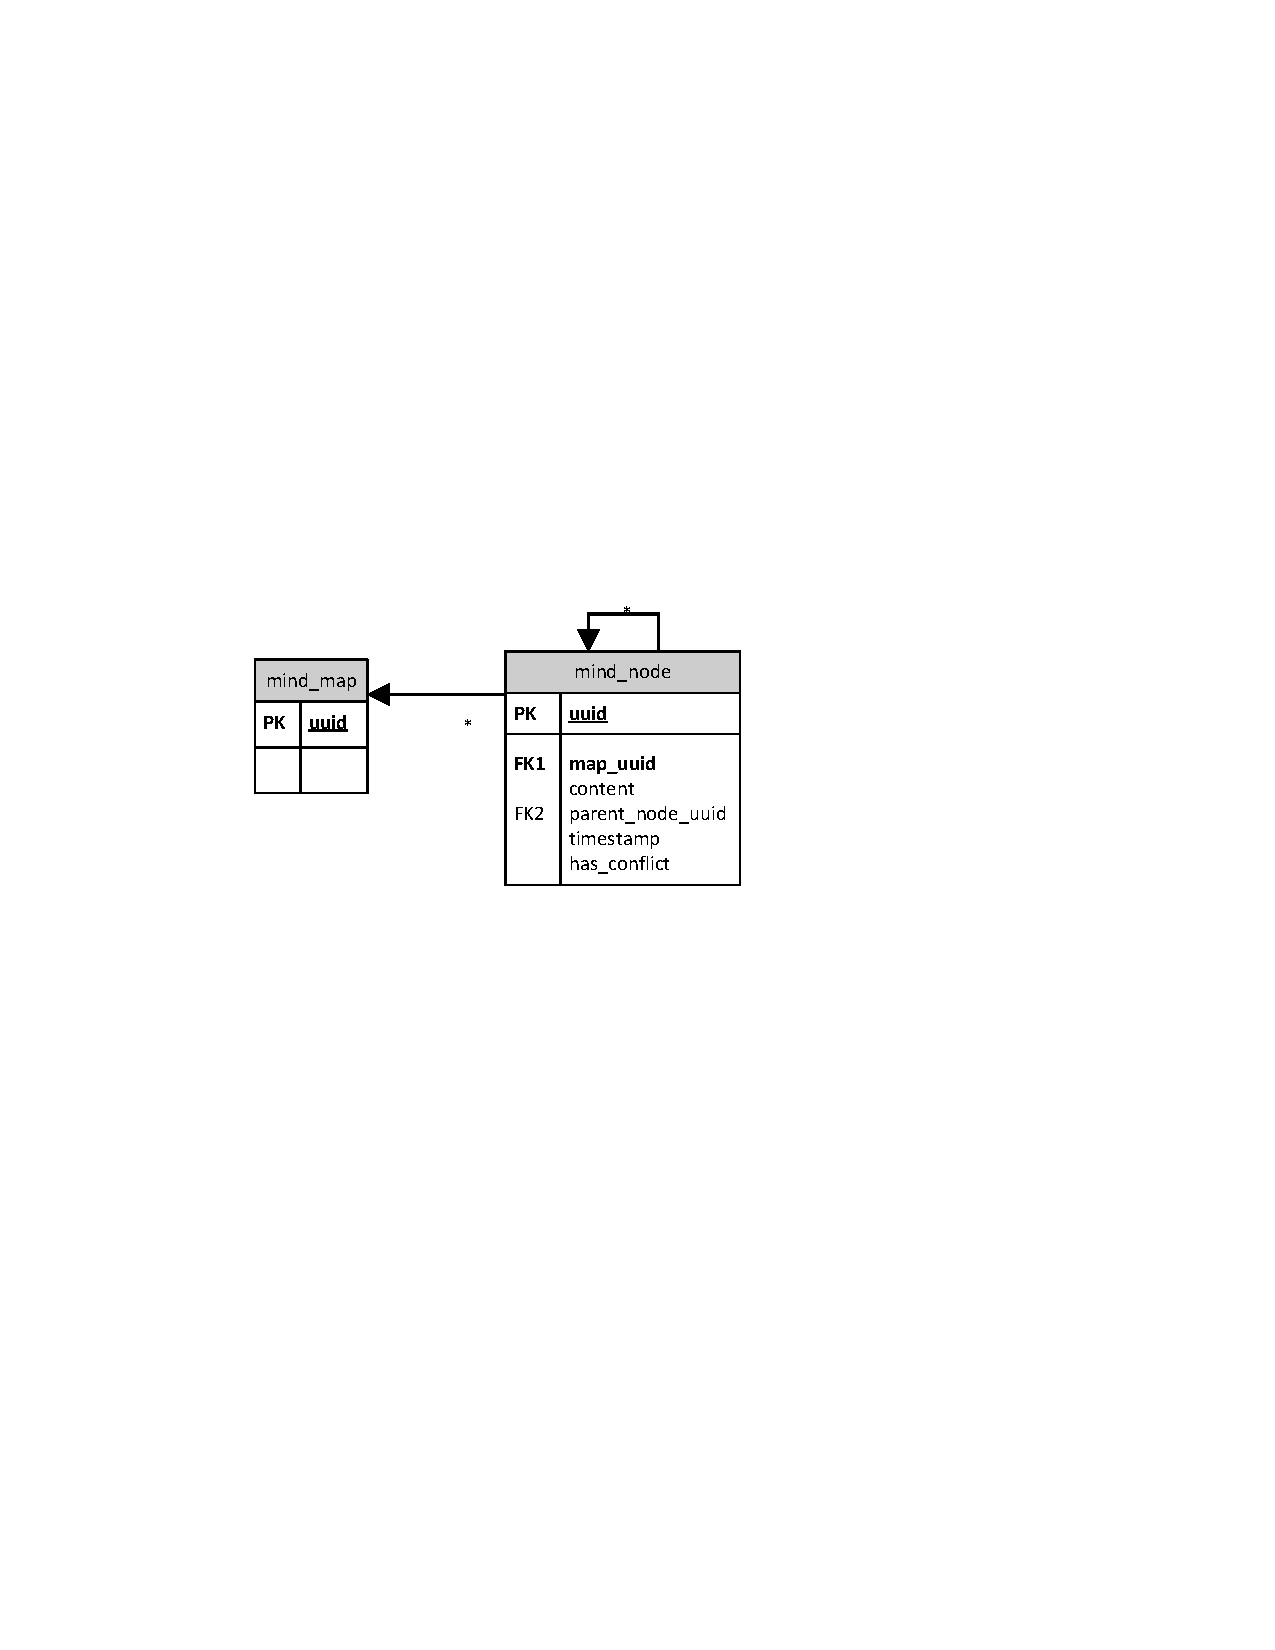
\includegraphics{graphics-erd}
	\caption{Entity relationship diagram of the database.}
	\label{fig:erd}
\end{figure}
